% Options for packages loaded elsewhere
\PassOptionsToPackage{unicode}{hyperref}
\PassOptionsToPackage{hyphens}{url}
%
\documentclass[
  8pt,
  ignorenonframetext,
]{beamer}
\usepackage{pgfpages}
\setbeamertemplate{caption}[numbered]
\setbeamertemplate{caption label separator}{: }
\setbeamercolor{caption name}{fg=normal text.fg}
\beamertemplatenavigationsymbolsempty
% Prevent slide breaks in the middle of a paragraph
\widowpenalties 1 10000
\raggedbottom
\setbeamertemplate{part page}{
  \centering
  \begin{beamercolorbox}[sep=16pt,center]{part title}
    \usebeamerfont{part title}\insertpart\par
  \end{beamercolorbox}
}
\setbeamertemplate{section page}{
  \centering
  \begin{beamercolorbox}[sep=12pt,center]{part title}
    \usebeamerfont{section title}\insertsection\par
  \end{beamercolorbox}
}
\setbeamertemplate{subsection page}{
  \centering
  \begin{beamercolorbox}[sep=8pt,center]{part title}
    \usebeamerfont{subsection title}\insertsubsection\par
  \end{beamercolorbox}
}
\AtBeginPart{
  \frame{\partpage}
}
\AtBeginSection{
  \ifbibliography
  \else
    \frame{\sectionpage}
  \fi
}
\AtBeginSubsection{
  \frame{\subsectionpage}
}
\usepackage{amsmath,amssymb}
\usepackage{lmodern}
\usepackage{iftex}
\ifPDFTeX
  \usepackage[T1]{fontenc}
  \usepackage[utf8]{inputenc}
  \usepackage{textcomp} % provide euro and other symbols
\else % if luatex or xetex
  \usepackage{unicode-math}
  \defaultfontfeatures{Scale=MatchLowercase}
  \defaultfontfeatures[\rmfamily]{Ligatures=TeX,Scale=1}
\fi
\usetheme[]{Copenhagen}
\usecolortheme{dolphin}
\usefonttheme{structurebold}
% Use upquote if available, for straight quotes in verbatim environments
\IfFileExists{upquote.sty}{\usepackage{upquote}}{}
\IfFileExists{microtype.sty}{% use microtype if available
  \usepackage[]{microtype}
  \UseMicrotypeSet[protrusion]{basicmath} % disable protrusion for tt fonts
}{}
\makeatletter
\@ifundefined{KOMAClassName}{% if non-KOMA class
  \IfFileExists{parskip.sty}{%
    \usepackage{parskip}
  }{% else
    \setlength{\parindent}{0pt}
    \setlength{\parskip}{6pt plus 2pt minus 1pt}}
}{% if KOMA class
  \KOMAoptions{parskip=half}}
\makeatother
\usepackage{xcolor}
\newif\ifbibliography
\usepackage{color}
\usepackage{fancyvrb}
\newcommand{\VerbBar}{|}
\newcommand{\VERB}{\Verb[commandchars=\\\{\}]}
\DefineVerbatimEnvironment{Highlighting}{Verbatim}{commandchars=\\\{\}}
% Add ',fontsize=\small' for more characters per line
\usepackage{framed}
\definecolor{shadecolor}{RGB}{248,248,248}
\newenvironment{Shaded}{\begin{snugshade}}{\end{snugshade}}
\newcommand{\AlertTok}[1]{\textcolor[rgb]{0.94,0.16,0.16}{#1}}
\newcommand{\AnnotationTok}[1]{\textcolor[rgb]{0.56,0.35,0.01}{\textbf{\textit{#1}}}}
\newcommand{\AttributeTok}[1]{\textcolor[rgb]{0.77,0.63,0.00}{#1}}
\newcommand{\BaseNTok}[1]{\textcolor[rgb]{0.00,0.00,0.81}{#1}}
\newcommand{\BuiltInTok}[1]{#1}
\newcommand{\CharTok}[1]{\textcolor[rgb]{0.31,0.60,0.02}{#1}}
\newcommand{\CommentTok}[1]{\textcolor[rgb]{0.56,0.35,0.01}{\textit{#1}}}
\newcommand{\CommentVarTok}[1]{\textcolor[rgb]{0.56,0.35,0.01}{\textbf{\textit{#1}}}}
\newcommand{\ConstantTok}[1]{\textcolor[rgb]{0.00,0.00,0.00}{#1}}
\newcommand{\ControlFlowTok}[1]{\textcolor[rgb]{0.13,0.29,0.53}{\textbf{#1}}}
\newcommand{\DataTypeTok}[1]{\textcolor[rgb]{0.13,0.29,0.53}{#1}}
\newcommand{\DecValTok}[1]{\textcolor[rgb]{0.00,0.00,0.81}{#1}}
\newcommand{\DocumentationTok}[1]{\textcolor[rgb]{0.56,0.35,0.01}{\textbf{\textit{#1}}}}
\newcommand{\ErrorTok}[1]{\textcolor[rgb]{0.64,0.00,0.00}{\textbf{#1}}}
\newcommand{\ExtensionTok}[1]{#1}
\newcommand{\FloatTok}[1]{\textcolor[rgb]{0.00,0.00,0.81}{#1}}
\newcommand{\FunctionTok}[1]{\textcolor[rgb]{0.00,0.00,0.00}{#1}}
\newcommand{\ImportTok}[1]{#1}
\newcommand{\InformationTok}[1]{\textcolor[rgb]{0.56,0.35,0.01}{\textbf{\textit{#1}}}}
\newcommand{\KeywordTok}[1]{\textcolor[rgb]{0.13,0.29,0.53}{\textbf{#1}}}
\newcommand{\NormalTok}[1]{#1}
\newcommand{\OperatorTok}[1]{\textcolor[rgb]{0.81,0.36,0.00}{\textbf{#1}}}
\newcommand{\OtherTok}[1]{\textcolor[rgb]{0.56,0.35,0.01}{#1}}
\newcommand{\PreprocessorTok}[1]{\textcolor[rgb]{0.56,0.35,0.01}{\textit{#1}}}
\newcommand{\RegionMarkerTok}[1]{#1}
\newcommand{\SpecialCharTok}[1]{\textcolor[rgb]{0.00,0.00,0.00}{#1}}
\newcommand{\SpecialStringTok}[1]{\textcolor[rgb]{0.31,0.60,0.02}{#1}}
\newcommand{\StringTok}[1]{\textcolor[rgb]{0.31,0.60,0.02}{#1}}
\newcommand{\VariableTok}[1]{\textcolor[rgb]{0.00,0.00,0.00}{#1}}
\newcommand{\VerbatimStringTok}[1]{\textcolor[rgb]{0.31,0.60,0.02}{#1}}
\newcommand{\WarningTok}[1]{\textcolor[rgb]{0.56,0.35,0.01}{\textbf{\textit{#1}}}}
\setlength{\emergencystretch}{3em} % prevent overfull lines
\providecommand{\tightlist}{%
  \setlength{\itemsep}{0pt}\setlength{\parskip}{0pt}}
\setcounter{secnumdepth}{-\maxdimen} % remove section numbering
\ifLuaTeX
  \usepackage{selnolig}  % disable illegal ligatures
\fi
\IfFileExists{bookmark.sty}{\usepackage{bookmark}}{\usepackage{hyperref}}
\IfFileExists{xurl.sty}{\usepackage{xurl}}{} % add URL line breaks if available
\urlstyle{same} % disable monospaced font for URLs
\hypersetup{
  pdftitle={Análisis de Datos Categóricos},
  pdfauthor={Ayudantía 3},
  hidelinks,
  pdfcreator={LaTeX via pandoc}}

\title{Análisis de Datos Categóricos}
\author{Ayudantía 3}
\date{Felipe Olivares}

\begin{document}
\frame{\titlepage}

\begin{frame}{Contenido}
\protect\hypertarget{contenido}{}
\begin{enumerate}
\item
  Funciones en R
\item
  Distribuciones binomial
\item
  Simulación de Monte Carlos
\item
  Gráficos en R
\end{enumerate}
\end{frame}

\begin{frame}{Funciones en R}
\protect\hypertarget{funciones-en-r}{}
Una función es un trozo de código autónomo que realiza una tarea
específica.

\begin{enumerate}
\item
  Las primeras son funciones que hacen algo y devuelven un objeto Estas
  funciones toman algunas entradas especificadas, hacen algunas
  manipulaciones / operaciones, y luego devuelven un objeto. Algunos
  ejemplos son \emph{mean()} (toma la media de un vector), \emph{lm()}
  (ajusta un modelo lineal), o \emph{read.csv} (carga una tabla de datos
  de formato excel).
\item
  En segundo lugar están las funciones que tienen algún efecto externo
  en su ordenador o entorno de trabajo. Estas funciones hacen algo pero
  no devuelven ningún objeto. Los ejemplos incluyen cosas como
  \emph{write.csv()} (escribe un archivo excel en tu computador),
  \emph{plot()} (hace un gráfico), \emph{library()} (carga un paquete).
\end{enumerate}
\end{frame}

\begin{frame}[fragile]{Funciones en R}
\protect\hypertarget{funciones-en-r-1}{}
Si bien la instalación de R base incorpora las funciones necesarias para
la estimación estadística y modelamiento de nuestros datos, en ocaciones
es común que necesitemos realizar tareas para las cuales el lenguaje no
ha especificado una función.

Veamos un ejemplo: El agua se congela a 0º Centígrados y hierve a 100º
Centígrados (diferencia de 100º). El agua se congela a 32º Fahrenheit y
hierve a 212º Fahrenheit (diferencia de 180º). Por lo tanto cada grado
en la escala Fahrenheit es igual a 100/180 o 5/9 grados en la escala
Celsius.

\begin{Shaded}
\begin{Highlighting}[]
 \CommentTok{\# Sintaxis}
\NormalTok{fahrenheit\_to\_celsius }\OtherTok{\textless{}{-}} \ControlFlowTok{function}\NormalTok{(temp\_F) \{}
\NormalTok{  temp\_C }\OtherTok{\textless{}{-}}\NormalTok{ (temp\_F }\SpecialCharTok{{-}} \DecValTok{32}\NormalTok{) }\SpecialCharTok{*} \DecValTok{5} \SpecialCharTok{/} \DecValTok{9}
  \FunctionTok{return}\NormalTok{(temp\_C)\}}
\end{Highlighting}
\end{Shaded}
\end{frame}

\begin{frame}[fragile]{Funciones en R}
\protect\hypertarget{funciones-en-r-2}{}
Ahora veamos los componentes de la función:

`fahrenheit\_to\_celsius' = nombre asignado a la función que será
ejecutada para llamarla.

function = comando que define argumentos y operaciones de la función.

() = argumentos de la función.

\{\} = operaciones de la función

\begin{Shaded}
\begin{Highlighting}[]
\CommentTok{\#Resultado}
\FunctionTok{fahrenheit\_to\_celsius}\NormalTok{ (}\DecValTok{32}\NormalTok{)}
\end{Highlighting}
\end{Shaded}

\begin{verbatim}
## [1] 0
\end{verbatim}
\end{frame}

\begin{frame}[fragile]{Distribución Binomial}
\protect\hypertarget{distribuciuxf3n-binomial}{}
Dentro de las distribuciones de probabilidad discretas, una de las más
populares es la distribución binomial. La simulación de variables
aleatorias que sigan parámetros de distribución Bernoulli y Binomial
puede ser ejecutadas a través de dos funciones incorporadas en R base.

\textbf{rbinom}: Esta función genera un vector de variables aleatorias
distribuidas binomialmente.

ejemplo: Obtener 1 cara con el lanzamiento de una moneda ``justa''

\begin{Shaded}
\begin{Highlighting}[]
\CommentTok{\# Sintaxis}
\NormalTok{ej1 }\OtherTok{\textless{}{-}} \FunctionTok{rbinom}\NormalTok{(}\AttributeTok{n=}\DecValTok{1}\NormalTok{, }\AttributeTok{size=}\DecValTok{1}\NormalTok{, }\AttributeTok{p=}\FloatTok{0.5}\NormalTok{)}
\NormalTok{ej1}
\end{Highlighting}
\end{Shaded}

\begin{verbatim}
## [1] 1
\end{verbatim}
\end{frame}

\begin{frame}[fragile]{Distribución Binomial}
\protect\hypertarget{distribuciuxf3n-binomial-1}{}
Donde los argumentos:

\textbf{n} = número de experimentos independientes.

\textbf{size} = número de intentos o teraciones.

\textbf{p} = probabilidad de éxito.

Otro ejemplo: Ahora tiramos la misma moneda ``justa'' 3 veces

\begin{Shaded}
\begin{Highlighting}[]
\FunctionTok{set.seed}\NormalTok{(}\DecValTok{12345}\NormalTok{)}
\NormalTok{ej2 }\OtherTok{\textless{}{-}} \FunctionTok{rbinom}\NormalTok{(}\AttributeTok{n=}\DecValTok{3}\NormalTok{, }\AttributeTok{size=}\DecValTok{1}\NormalTok{, }\AttributeTok{p=}\FloatTok{0.5}\NormalTok{) }
\NormalTok{ej2}
\end{Highlighting}
\end{Shaded}

\begin{verbatim}
## [1] 1 1 1
\end{verbatim}
\end{frame}

\begin{frame}{Distribución Binomial}
\protect\hypertarget{distribuciuxf3n-binomial-2}{}
\textbf{dbinom}: Esta función devuelve el valor de la función de
densidad de probabilidad.

tomemos el caso de una moneda justa para una probabilidad de obtener 5
caras con 10 lanzamientos

\[\mathbb{P}(Y=5) =  \frac{10!}{5! 5!} \times (0.5)^{5} \times (1-0.5)^{5} = 252 \times (0.5)^{10} = 0.25\]
\end{frame}

\begin{frame}[fragile]{Distribución Binomial}
\protect\hypertarget{distribuciuxf3n-binomial-3}{}
Veamos ahora el código en \emph{R}

\begin{Shaded}
\begin{Highlighting}[]
\CommentTok{\#  obtener 5 "Caras" con 10 lanzamientos}
\NormalTok{ej3 }\OtherTok{\textless{}{-}} \FunctionTok{dbinom}\NormalTok{(}\AttributeTok{x=}\DecValTok{5}\NormalTok{,}\AttributeTok{size=}\DecValTok{10}\NormalTok{,}\AttributeTok{prob=}\FloatTok{0.5}\NormalTok{)}
\NormalTok{ej3}
\end{Highlighting}
\end{Shaded}

\begin{verbatim}
## [1] 0.2460938
\end{verbatim}

Donde los argumentos:

x = número de éxitos.

size = número de intentos o teraciones.

p = probabilidad de éxito.
\end{frame}

\begin{frame}[fragile]{Distribución Binomial}
\protect\hypertarget{distribuciuxf3n-binomial-4}{}
Veamos otro ejemplo:

La función \textbf{dbinom} devuelve el valor de la función de densidad
de probabilidad de la distribución binomial dada una determinada
variable aleatoria ``\emph{x}'' , número de ensayos ``\emph{size}''
(tamaño de la muestra) y probabilidad de éxito en cada ensayo
``\emph{prob}''

Carlos cuando juega fútbol acerta el 80\% de sus penales. Si lanza 12
penales, ¿cuál es la probabilidad de que haga exactamente 10?

\begin{Shaded}
\begin{Highlighting}[]
\CommentTok{\# Sintaxis}
\NormalTok{ej4 }\OtherTok{\textless{}{-}} \FunctionTok{dbinom}\NormalTok{(}\AttributeTok{x=}\DecValTok{10}\NormalTok{,}\AttributeTok{size=}\DecValTok{12}\NormalTok{,}\AttributeTok{prob=}\FloatTok{0.8}\NormalTok{)}
\NormalTok{ej4}
\end{Highlighting}
\end{Shaded}

\begin{verbatim}
## [1] 0.2834678
\end{verbatim}
\end{frame}

\begin{frame}[fragile]{Simulación de Monte Carlo}
\protect\hypertarget{simulaciuxf3n-de-monte-carlo}{}
La simulación o método de Montecarlo es un método estadístico utilizado
para resolver problemas matemáticos complejos a través de la generación
de variables aleatorias. Método de Monte Carlo o una simulación de
probabilidad múltiple, es una técnica matemática que se utiliza para
estimar los posibles resultados de un evento incierto. Una simulación de
Monte Carlo crea un modelo de posibles resultados aprovechando una
distribución de probabilidades, por ejemplo, una distribución binomial.

supongamos que tenemos 2 monedas sesgadas con una probabilidad de que
salga cara de un 40\% y otra de 60\%

\begin{Shaded}
\begin{Highlighting}[]
\FunctionTok{set.seed}\NormalTok{(}\DecValTok{12345}\NormalTok{) }\CommentTok{\#limpiar para randomización}

\CommentTok{\#Monedas sesgadas}
\NormalTok{moneda1 }\OtherTok{\textless{}{-}} \FunctionTok{rep}\NormalTok{(}\FunctionTok{c}\NormalTok{(}\StringTok{"Cara"}\NormalTok{, }\StringTok{"Sello"}\NormalTok{), }\AttributeTok{times =} \FunctionTok{c}\NormalTok{(}\DecValTok{4}\NormalTok{, }\DecValTok{6}\NormalTok{)) }\CommentTok{\# \%40}
\NormalTok{moneda2 }\OtherTok{\textless{}{-}} \FunctionTok{rep}\NormalTok{(}\FunctionTok{c}\NormalTok{(}\StringTok{"Cara"}\NormalTok{, }\StringTok{"Sello"}\NormalTok{), }\AttributeTok{times =} \FunctionTok{c}\NormalTok{(}\DecValTok{6}\NormalTok{, }\DecValTok{4}\NormalTok{)) }\CommentTok{\# \%60}

\CommentTok{\#simulamos un experimento donde tiramos 100000 veces la moneda}
\NormalTok{num\_veces }\OtherTok{\textless{}{-}} \DecValTok{100000} 
\NormalTok{resultado1 }\OtherTok{\textless{}{-}} \FunctionTok{replicate}\NormalTok{(num\_veces, \{}
  \FunctionTok{sample}\NormalTok{(moneda1, }\DecValTok{1}\NormalTok{) \})}
\NormalTok{resultado2 }\OtherTok{\textless{}{-}} \FunctionTok{replicate}\NormalTok{(num\_veces, \{}
  \FunctionTok{sample}\NormalTok{(moneda2, }\DecValTok{1}\NormalTok{)\})}
\end{Highlighting}
\end{Shaded}
\end{frame}

\begin{frame}[fragile]{Simulación de Monte Carlo}
\protect\hypertarget{simulaciuxf3n-de-monte-carlo-1}{}
\(\mathbb{P}(C_{1}C_{2}) = \mathbb{P}(C_{1})\mathbb{P}(C_{2}) = 0.4 \times 0.6 = 0.24\)

\begin{Shaded}
\begin{Highlighting}[]
\FunctionTok{table}\NormalTok{(resultado1)}
\end{Highlighting}
\end{Shaded}

\begin{verbatim}
## resultado1
##  Cara Sello 
## 40138 59862
\end{verbatim}

\begin{Shaded}
\begin{Highlighting}[]
\FunctionTok{table}\NormalTok{(resultado2)}
\end{Highlighting}
\end{Shaded}

\begin{verbatim}
## resultado2
##  Cara Sello 
## 60002 39998
\end{verbatim}

\begin{Shaded}
\begin{Highlighting}[]
\CommentTok{\#promedio}
\NormalTok{a}\OtherTok{\textless{}{-}}\FunctionTok{mean}\NormalTok{(moneda1}\SpecialCharTok{==}\StringTok{"Cara"}\NormalTok{)}
\NormalTok{b}\OtherTok{\textless{}{-}}\FunctionTok{mean}\NormalTok{(moneda2}\SpecialCharTok{==}\StringTok{"Cara"}\NormalTok{)}

\CommentTok{\#test deindependencia}
\NormalTok{a }\SpecialCharTok{*}\NormalTok{ b}
\end{Highlighting}
\end{Shaded}

\begin{verbatim}
## [1] 0.24
\end{verbatim}
\end{frame}

\begin{frame}{Gráficos}
\protect\hypertarget{gruxe1ficos}{}
Una de las herramientas más útiles para la exploración y evaluación de
nuestros datos son los análisis visuales disponibles a partir de
distintas funciones de R. Con todo, uno de los repositorios más útiles y
de más alta potencia gráfica es library(ggplot2) el cual forma parte de
las funciones incluidas en la librería library(tidyverse).

A continuación veamos una breve introducción a su sintaxis y usos.
\end{frame}

\begin{frame}{Gráficos}
\protect\hypertarget{gruxe1ficos-1}{}
Existen 3 elementos centrales en la sintaxis del comando ggplot:

\begin{enumerate}
\item
  Una estructura visual (aesthetic) que le informa a ggplot qué
  variables serán mapeadas en el eje X e Y, (y frecuentemente otros
  atributos del gráfico, como los esquemas de color con que serán
  completados). Intuitivamente, aes puede ser pensada como la función
  que especifica qué estarás graficando.
\item
  Una geometría (geom) que le informa a ggplot cuál será la estructura
  básica para la creación del gráfico. Intuitivamente, geom puede ser
  pensada como la función que especifica cómo estarás graficando.
\item
  Otras opciones de customización (labels), como los títulos del
  gráfico, los tamaños de los elementos, el tipo de tema de
  construcción, etc. En la función esto es conocido como labs.
\end{enumerate}

Entonces:

\begin{itemize}
\tightlist
\item
  \textbf{ggplot= aes + geom + labs}
\end{itemize}
\end{frame}

\begin{frame}[fragile]{Gráficos}
\protect\hypertarget{gruxe1ficos-2}{}
Utilizando la base de datos del Observatorio de conflictos de COES.
Observemos la presencia de organizaciones sociales para el conjunto de
los datos 2009-2019

\begin{Shaded}
\begin{Highlighting}[]
\CommentTok{\# Sintaxis gráficos de barras}
\FunctionTok{ggplot}\NormalTok{(df1, }\FunctionTok{aes}\NormalTok{(}\AttributeTok{x =}\NormalTok{ organizacion)) }\SpecialCharTok{+} \CommentTok{\# definimos eje X }
  \FunctionTok{geom\_bar}\NormalTok{() }\SpecialCharTok{+}  \CommentTok{\# gráficos de barras básico}
  \FunctionTok{labs}\NormalTok{(}\AttributeTok{title =} \StringTok{"OCS 2009{-}2019"}\NormalTok{,}
       \AttributeTok{subtitle =} \StringTok{"Gráficos de barras organizaciones"}\NormalTok{, }
       \AttributeTok{caption =} \StringTok{"Figura 1"}\NormalTok{, }\AttributeTok{x =} \StringTok{"Organizaciones"}\NormalTok{, }\AttributeTok{y =} \StringTok{"conteo"}\NormalTok{)}
\end{Highlighting}
\end{Shaded}

\begin{center}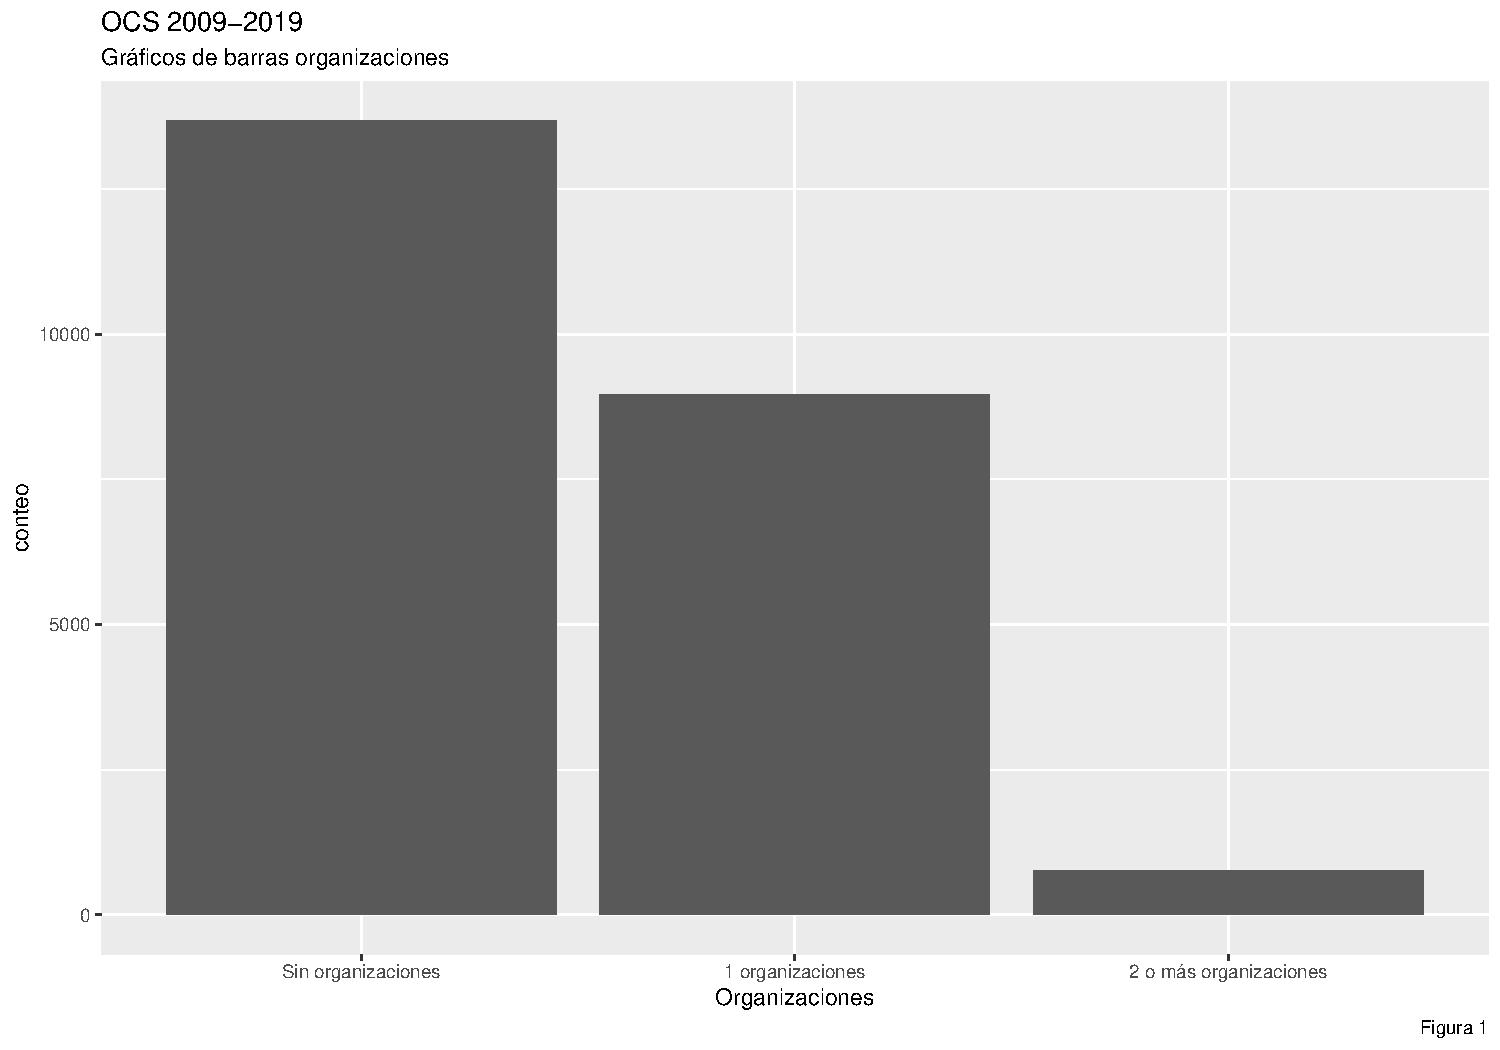
\includegraphics[width=0.7\linewidth]{ta_3_files/figure-beamer/unnamed-chunk-10-1} \end{center}
\end{frame}

\begin{frame}[fragile]{Gráficos}
\protect\hypertarget{gruxe1ficos-3}{}
Otro ejemplo puede ser tomar las protestas laborales y ver la ocurrencia
en el tiempo

\begin{Shaded}
\begin{Highlighting}[]
\CommentTok{\#trabajamos los datos}
\NormalTok{df\_lab }\OtherTok{\textless{}{-}}\NormalTok{ df1 }\SpecialCharTok{\%\textgreater{}\%} \FunctionTok{filter}\NormalTok{(laboral }\SpecialCharTok{==} \StringTok{"Sí"}\NormalTok{) }\SpecialCharTok{\%\textgreater{}\%} \CommentTok{\# protestas laborales}
  \FunctionTok{group\_by}\NormalTok{(ano) }\SpecialCharTok{\%\textgreater{}\%} \CommentTok{\#agrupamos por año}
   \FunctionTok{summarise}\NormalTok{(}\AttributeTok{frecuencia =} \FunctionTok{n}\NormalTok{()) }\SpecialCharTok{\%\textgreater{}\%} \CommentTok{\# contamos las frecuencias anuales}
  \FunctionTok{mutate}\NormalTok{(}\AttributeTok{demanda =} \StringTok{"laboral"}\NormalTok{) }\CommentTok{\#creamos la variable }

\FunctionTok{head}\NormalTok{ (df\_lab)}
\end{Highlighting}
\end{Shaded}

\begin{verbatim}
## # A tibble: 6 x 3
##   ano   frecuencia demanda
##   <fct>      <int> <chr>  
## 1 2009         787 laboral
## 2 2010         525 laboral
## 3 2011         433 laboral
## 4 2012         445 laboral
## 5 2013        1006 laboral
## 6 2014         955 laboral
\end{verbatim}
\end{frame}

\begin{frame}[fragile]{Gráficos}
\protect\hypertarget{gruxe1ficos-4}{}
\begin{Shaded}
\begin{Highlighting}[]
\CommentTok{\# Sintaxis gráficos de lineas}
 \FunctionTok{ggplot}\NormalTok{(df\_lab, }\FunctionTok{aes}\NormalTok{(}\AttributeTok{x =}\NormalTok{ ano, }\AttributeTok{y =}\NormalTok{ frecuencia,}\AttributeTok{group =} \DecValTok{1}\NormalTok{, }\AttributeTok{colour =}\NormalTok{ demanda))}\SpecialCharTok{+}
   \FunctionTok{geom\_line}\NormalTok{()}\SpecialCharTok{+} \CommentTok{\#gráficos de lineas}
   \FunctionTok{coord\_cartesian}\NormalTok{(}\AttributeTok{ylim=}\FunctionTok{c}\NormalTok{(}\DecValTok{0}\NormalTok{,}\DecValTok{1200}\NormalTok{)) }\SpecialCharTok{+} \CommentTok{\# coordenadas del eje Y}
  \FunctionTok{labs}\NormalTok{(}\AttributeTok{title =} \StringTok{\textquotesingle{}Frecuencias demandas laborales\textquotesingle{}}\NormalTok{,  }
       \AttributeTok{y =} \StringTok{\textquotesingle{}Frecuencias\textquotesingle{}}\NormalTok{, }
       \AttributeTok{x =} \StringTok{\textquotesingle{}Demandas laborales\textquotesingle{}}\NormalTok{,}
       \AttributeTok{colour =} \StringTok{\textquotesingle{}Demandas\textquotesingle{}}\NormalTok{)}
\end{Highlighting}
\end{Shaded}

\begin{center}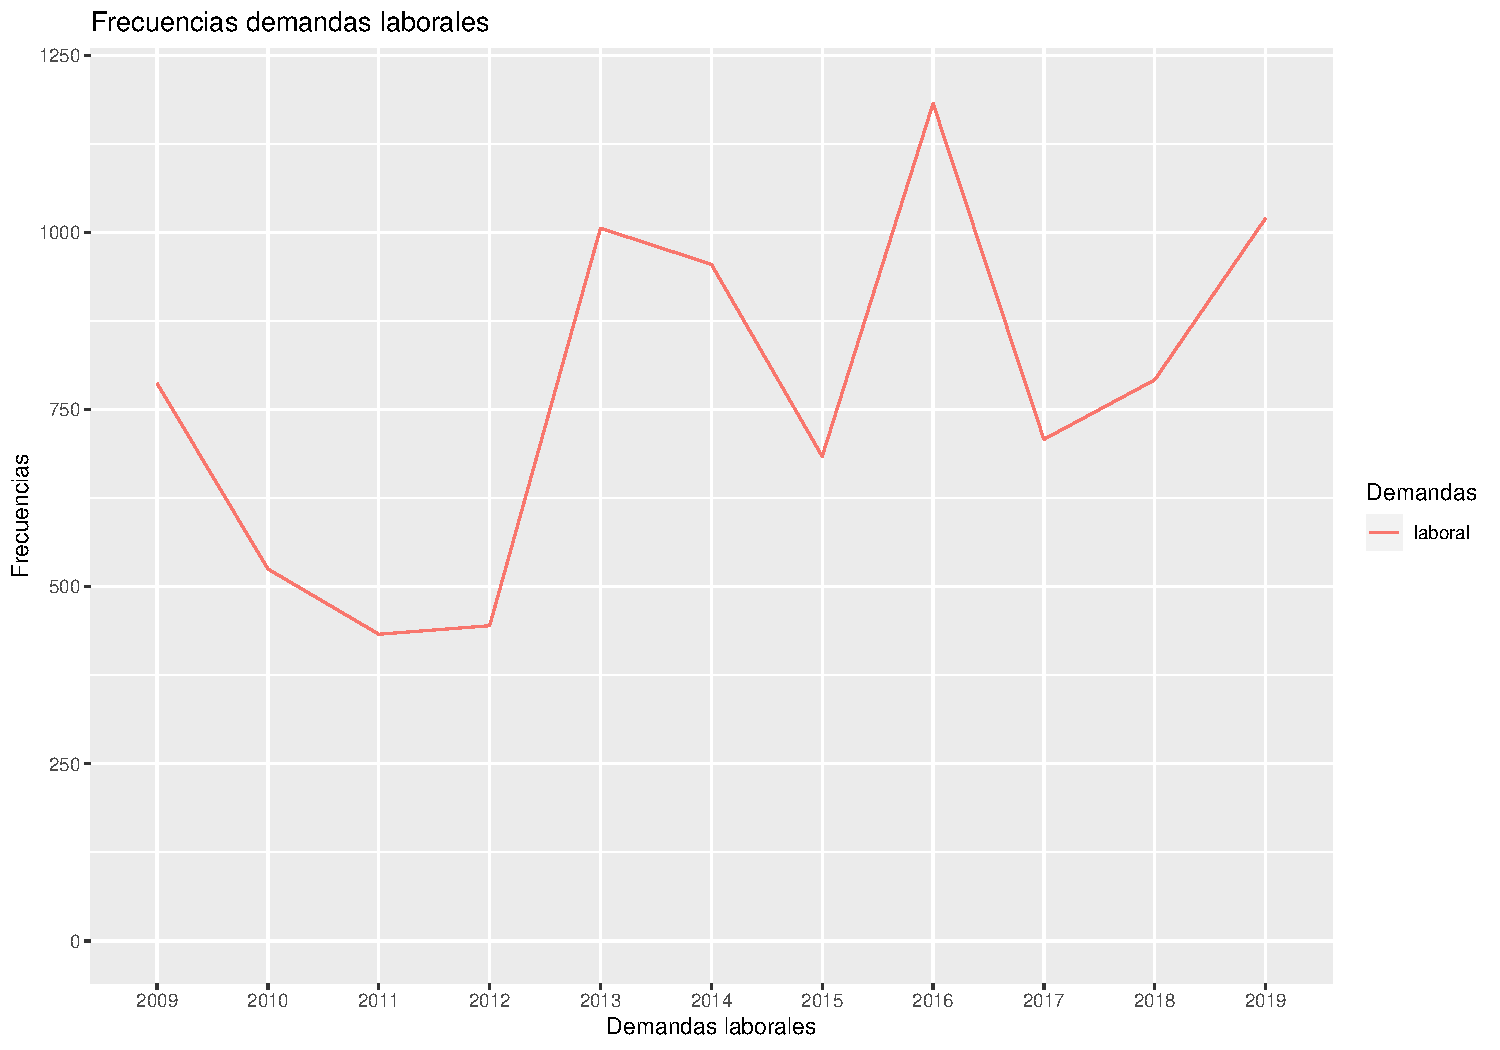
\includegraphics[width=0.7\linewidth]{ta_3_files/figure-beamer/unnamed-chunk-12-1} \end{center}
\end{frame}

\begin{frame}[fragile]{Gráficos}
\protect\hypertarget{gruxe1ficos-5}{}
\begin{Shaded}
\begin{Highlighting}[]
\CommentTok{\#Sintaxis gráficos de barras}
\NormalTok{g1 }\OtherTok{\textless{}{-}}\NormalTok{df1 }\SpecialCharTok{\%\textgreater{}\%} \FunctionTok{group\_by}\NormalTok{(macrozona) }\SpecialCharTok{\%\textgreater{}\%} \CommentTok{\# guardamos el gráfico en "g1"}
  \FunctionTok{count}\NormalTok{(violenta) }\SpecialCharTok{\%\textgreater{}\%}  \CommentTok{\#contamos las tácticas violentas}
  \FunctionTok{mutate}\NormalTok{(}\AttributeTok{prop =} \FunctionTok{prop.table}\NormalTok{(n)) }\SpecialCharTok{\%\textgreater{}\%}  \CommentTok{\#sacamos el \%}
  \FunctionTok{ggplot}\NormalTok{(}\FunctionTok{aes}\NormalTok{(}\AttributeTok{x =}\NormalTok{ violenta, }\AttributeTok{y =}\NormalTok{ prop,}
             \AttributeTok{fill=}\NormalTok{macrozona, }\AttributeTok{label=}\NormalTok{scales}\SpecialCharTok{::}\FunctionTok{percent}\NormalTok{(prop, }\AttributeTok{accuracy =}\NormalTok{.}\DecValTok{1}\NormalTok{))) }\SpecialCharTok{+}
  \FunctionTok{geom\_bar}\NormalTok{(}\AttributeTok{stat=}\StringTok{"identity"}\NormalTok{, }\AttributeTok{width=}\FloatTok{0.8}\NormalTok{, }\AttributeTok{position =} \StringTok{"dodge"}\NormalTok{)}\SpecialCharTok{+}  
  \FunctionTok{coord\_flip}\NormalTok{(}\AttributeTok{ylim =}\FunctionTok{c}\NormalTok{(}\DecValTok{0}\NormalTok{,}\DecValTok{1}\NormalTok{)) }\SpecialCharTok{+} \CommentTok{\#rotamos el gráfico}
  \FunctionTok{labs}\NormalTok{(}\AttributeTok{title =} \StringTok{\textquotesingle{}Porcentaje de tácticas violentas según macrozona\textquotesingle{}}\NormalTok{, }
       \AttributeTok{y =} \StringTok{\textquotesingle{}Porcentaje\textquotesingle{}}\NormalTok{, }
       \AttributeTok{x =} \StringTok{\textquotesingle{}Tácticas violentas\textquotesingle{}}\NormalTok{,}
       \AttributeTok{fill =} \StringTok{\textquotesingle{}Macrozonas\textquotesingle{}}\NormalTok{)}\SpecialCharTok{+} 
  \FunctionTok{theme}\NormalTok{(}\AttributeTok{axis.title =} \FunctionTok{element\_text}\NormalTok{(), }\AttributeTok{text =} \FunctionTok{element\_text}\NormalTok{(}\AttributeTok{size =} \DecValTok{12}\NormalTok{))}\SpecialCharTok{+}
   \FunctionTok{geom\_text}\NormalTok{(}\AttributeTok{position =} \FunctionTok{position\_dodge2}\NormalTok{(}\AttributeTok{width =}\NormalTok{ .}\DecValTok{9}\NormalTok{), }\CommentTok{\# colocamos los \%     }
              \AttributeTok{vjust =} \FloatTok{0.35}\NormalTok{,}
              \AttributeTok{hjust =} \SpecialCharTok{{-}}\FloatTok{0.8}\NormalTok{,}
              \AttributeTok{size =} \DecValTok{3}\NormalTok{)}
\end{Highlighting}
\end{Shaded}
\end{frame}

\begin{frame}[fragile]{Gráficos}
\protect\hypertarget{gruxe1ficos-6}{}
\begin{Shaded}
\begin{Highlighting}[]
\CommentTok{\#llamamos el gráfico creado}
\NormalTok{g1}
\end{Highlighting}
\end{Shaded}

\begin{center}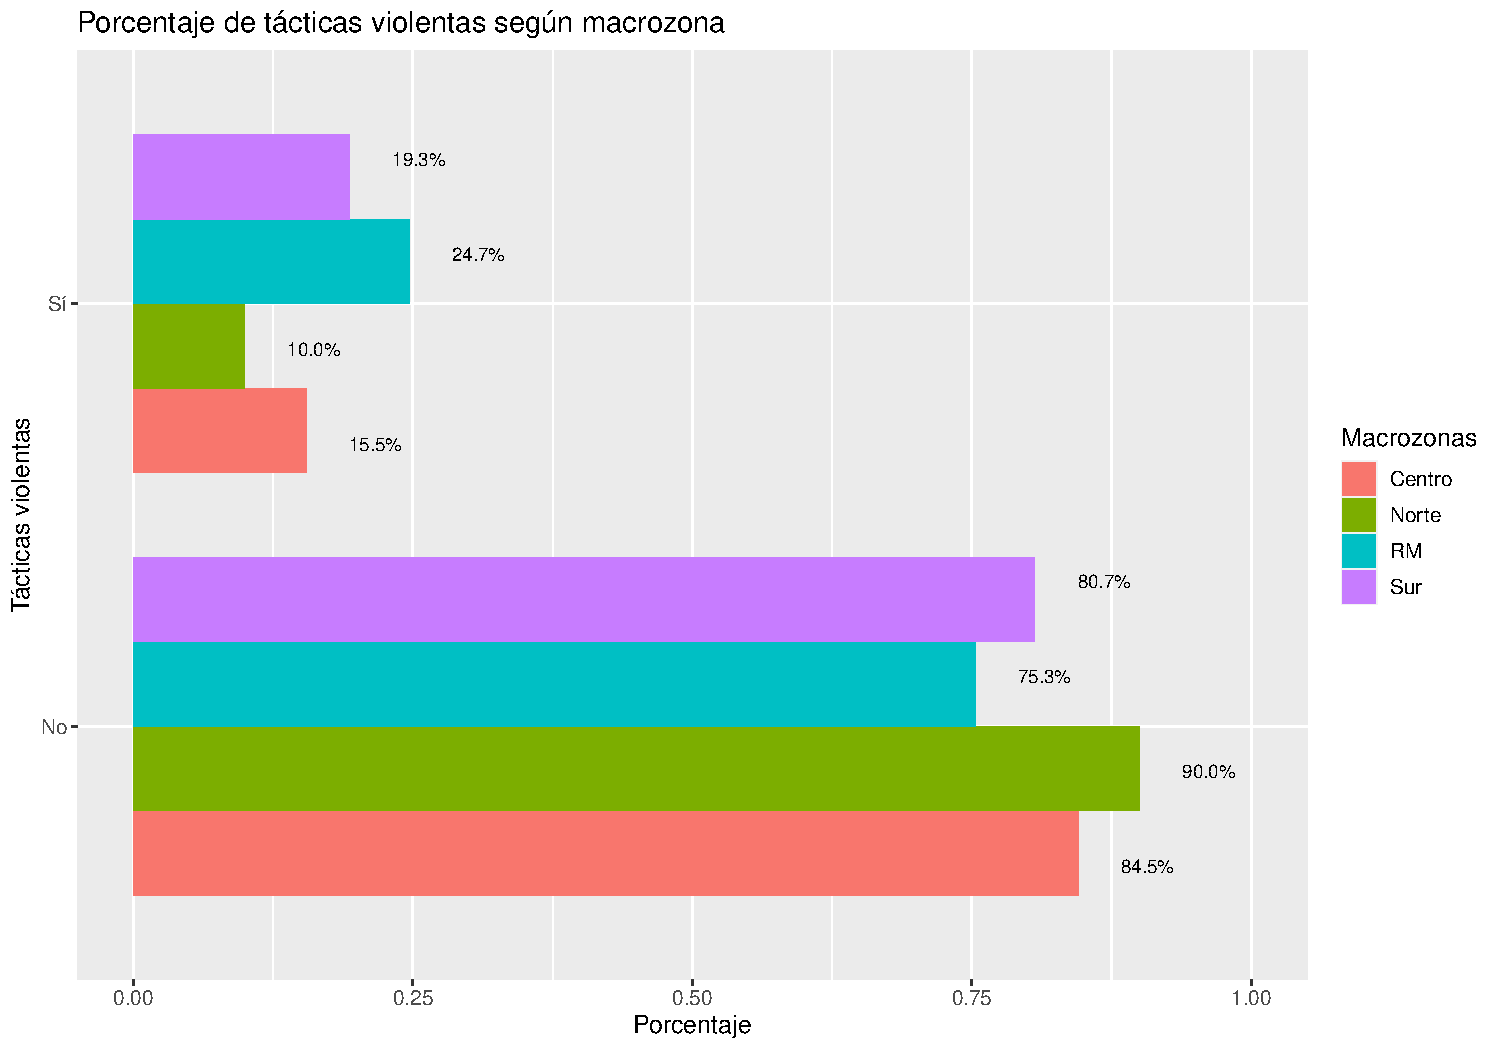
\includegraphics[width=0.9\linewidth]{ta_3_files/figure-beamer/unnamed-chunk-14-1} \end{center}
\end{frame}

\begin{frame}{Consejos}
\protect\hypertarget{consejos}{}
\begin{enumerate}
\item
  El aprendizaje de R es como la práctica de un instrumento musical,
  entre \textbf{mayor dedicación y frecuencia de práctica mejor será la
  adaptación al programa, su uso y fluidez.} Recomendamos explorar
  RStudio y el lenguaje R todas las semanas para apoyar el aprendizaje
  progresivo.
\item
  Al ser parte de una \textbf{comunidad académica internacional}, muchas
  de las dudas que puedas tener en el camino son y han sido discutidas
  en múltiples recursos de internet como \textbf{blogs, foros, y
  tutoriales} que dan soluciones múltiples a un mismo problema. A modo
  de apoyo es recomendado consultar los recursos disponibles en internet
  además del material de ayudantías y consultas del curso.
\end{enumerate}
\end{frame}

\end{document}
